\renewcommand{\theequation}{\theenumi}
\renewcommand{\thefigure}{\theenumi}
\begin{enumerate}[label=\thesection.\arabic*.,ref=\thesection.\theenumi]
\numberwithin{equation}{enumi}
\numberwithin{figure}{enumi}
\numberwithin{table}{enumi}
\item The joint probability density function of (X,Y) is
\begin{equation}
    f(x,y) =
    \begin{cases}
        6(1-x) & if \hspace{0.3cm}0<y<x ,0<x<1\label{0.0.1} \\
        0      & \text{otherwise}
    \end{cases}
\end{equation}
Which among the following are correct?
\begin{enumerate}\itemsep0.3cm
    \item X and Y are not independent
    \item
          $ f_Y(y) =
              \begin{cases}
                  3\brak{y-1}^{2} & if \hspace{0.3cm}0<y<1 \\
                  0               & \text{otherwise}
              \end{cases}$
    \item X and Y are independent
    \item $ f_Y(y) =
              \begin{cases}
                  3\brak{\displaystyle{y-\frac{1}{2}{y}^2}} & if \hspace{0.3cm}0<y<1 \\
                  0                                         & \text{otherwise}
              \end{cases}$
\end{enumerate}
%
\solution
Given joint probability density function of X and Y, marginal probability density functions are as follows:
\begin{align}
    f_X(x) = \int_{-\infty}^{\infty} f(x,y) dy \\[0.4cm]
    f_Y(y) = \int_{-\infty}^{\infty} f(x,y) dx
\end{align}
Calculating $f_X(x)$
\begin{align}
    f_X(x) = & \int_{-\infty}^{\infty} f(x,y) dy \\
    =        & \int_{0}^{x} 6(1-x) dy            
\end{align}
\begin{align}
    f_X(x) =
    \begin{cases}
        6x(1-x) & 0<x<1     \label{june2016-104:0.0.6}\\
        0       & otherwise
    \end{cases}
\end{align}
Calculating $f_Y(y)$
\begin{align}
    f_Y(y) = & \int_{-\infty}^{\infty} f(x,y) dx \\
    =        & \int_{y}^{1} 6(1-x) dx\\
    =        & 6x -3{x}^2 \big|_{y}^{1}\\
    =        & 3 - 6y + 3y^{2}\\
    =        & 3{(y-1)}^{2}      
\end{align}
\begin{align}
    f_Y(y) =
    \begin{cases}
        3{(y-1)}^{2}  & 0<y<1     \label{june2016-104:0.0.12}\\
        0       & otherwise
    \end{cases}
\end{align}
To check whether X and Y are independent, we calculate $f_X(x) \times f_Y(y)$. From \eqref{june2016-104:0.0.6} and \eqref{june2016-104:0.0.12}
\begin{align}
    f_X(x) \times f_Y(y) = &
    \begin{cases}
        18x(1-x){(y-1)}^{2}  \\ \hspace{1.2cm}0<x<1,0<y<1\\
        0 \hspace{1cm} \text{otherwise}
    \end{cases}\\
    \neq & f(x,y)
\end{align}
Since f(x,y) and $f_X(x)\times f_Y(y)$ are different, random variables X and Y are not independent.
\begin{center}
    Options 1 and 2 are correct
\end{center}
%
\item Three types of components are used in electrical circuits 1, 2, 3 as shown below in the figure
\begin{figure}[h]
    \centering
    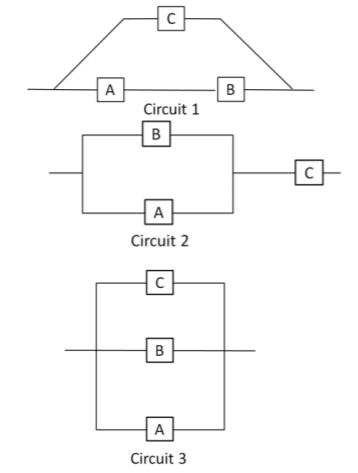
\includegraphics[width=\columnwidth]{solutions/2016/june/118/Figures/circuits.png}
    \caption{Figure}
    \label{fig:fig_label}
\end{figure}
%
\solution
For $q_1$, the truth table
\begin{table}[h]
    \centering
    \begin{tabular}{|c|c|c|c|}
    \hline
         $A$ & $B$ & $C$ & $(AB) + C$ \\
         \hline
         1 &1  & 0 &1\\\hline
         1&1&1&1\\\hline
         0&1&1&1\\\hline
         0&0&1&1\\\hline
         1&0&1&1\\
    \hline
    \end{tabular}
    \caption{Circuit 1 working}
    \label{june2016-118:tab:my_label}
\end{table}
Multiplying and adding probability for each case of $q_1$ gives us the value of $q_1$ as
\begin{align}
    q_1 = p^3-2p^2+1
\end{align}
For $q_2$, the truth table
\begin{table}[h]
    \centering
    \begin{tabular}{|c|c|c|c|}
    \hline
         $A$ & $B$ & $C$ & $(A+B)C$ \\
         \hline
         1&1&1&1\\ \hline
         1&0&1&1\\\hline
         0&1&1&1\\
    \hline
    \end{tabular}
    \caption{Circuit 2 working}
    \label{june2016-118:tab:table2}
\end{table}
Multiplying and adding probability for each case of $q_2$ gives us the value of $q_2$ as
\begin{align}
    q_2 = p^3-p^2-p+1
\end{align}
For $q_3$, the truth table
\begin{table}[h]
    \centering
    \begin{tabular}{|c|c|c|c|}
    \hline
         $A$ & $B$ & $C$ & $A + B + C$ \\
         \hline
         1&0&0&1\\\hline
         0&1&0&1\\\hline
         0&0&1&1\\\hline
         1&1&0&1\\\hline
         1&0&1&1\\\hline
         0&1&1&1\\\hline
         1&1&1&1\\
    \hline
    \end{tabular}
    \caption{Circuit 3 working}
    \label{june2016-118:tab:table3}
\end{table}
Multiplying and adding probability for each case of $q_3$ gives us the value of $q_3$ as
\begin{align}
    q_3 = 1-p^3
\end{align}
%%
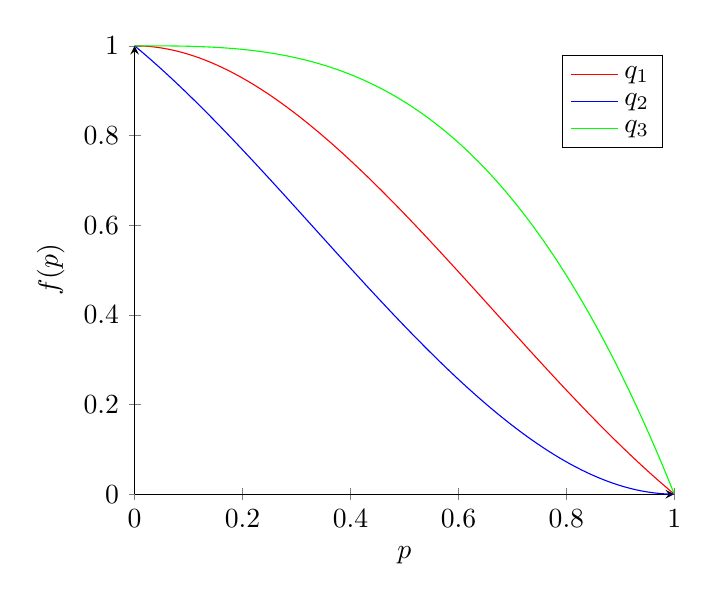
\begin{tikzpicture}
\begin{axis}[
    axis lines = left,
    xlabel = $p$,
    ylabel = {$f(p)$},
]
\addplot [
    domain=0:1, 
    samples=100, 
    color=red,
]
{x^3-2*x^2+1};
\addlegendentry{$q_1$}
\addplot [
    domain=0:1, 
    samples=100, 
    color=blue,
    ]
    {x^3-x^2-x+1};
\addlegendentry{$q_2$}
\addplot [
    domain=0:1, 
    samples=100, 
    color=green,
]
{1-x^3};
\addlegendentry{$q_3$}
\end{axis}
\end{tikzpicture}
\begin{align}
    \therefore q_3>q_1>q_2
\end{align}
Hence \textbf{Option 1} is correct
%
\item Suppose X and Y are independent and identically distributed random variables and let $Z = X + Y$. Then the distribution of $Z$ is in the same family as that of $X$ and $Y$ if X is
\begin{table}[h]
\setlength{\tabcolsep}{30pt}
    \begin{tabular}{ll}
         1) Normal  & 2) Exponential  \\
         3) Uniform & 4) Binomial
    \end{tabular}
\end{table}
%
\solution


\begin{enumerate}[label = \arabic*)]
    \item Let X and Y be independent and identically distributed normal random variables. Then the characteristic function of X and Y is given by
    \begin{equation}
        \Phi_X(\omega) = e^{j\eta\omega - \sigma^2\omega^2/2}
    \end{equation}
    The characteristic function of Z is given by
    \begin{align}
        \Phi_Z(\omega) &= \Phi_X^2(\omega)\\
                       &= e^{2j\eta\omega - \sigma^2\omega^2}
    \end{align}
    Thus Z is a normal random variable with parameters $2\eta$ and $2\sigma^2$. Thus option (1) is correct.
    \item Let X and Y be independent and identically distributed exponential random variables. Then the characteristic function of X and Y is given by
    \begin{equation}
        \Phi_X(\omega) = \dfrac{\lambda}{1-j\omega}
    \end{equation}
    The characteristic function of Z is given by
    \begin{align}
        \Phi_Z(\omega) &= \Phi_X^2(\omega)\\
                       &= \dfrac{\lambda^2}{(1-j\omega)^2}
    \end{align}
    Thus Z is not an exponential random variable. Therefore option (2) is wrong.
    \item Let X and Y be independent and identically distributed uniform random variables such that X, Y $\sim$ U(a,b). Then the characteristic function of X and Y is given by
    \begin{equation}
        \Phi_X(\omega) = \dfrac{e^{jb\omega} - e^{ja\omega}}{j\omega(b-a)}
    \end{equation}
    The characteristic function of Z is given by
    \begin{align}
        \Phi_Z(\omega) &= \Phi_X^2(\omega)\\
                       &= -\dfrac{(e^{jb\omega} - e^{ja\omega})^2}{\omega^2(b-a)^2}
    \end{align}
    Thus Z is not a uniform random variable. Thus option (3) is wrong.
    \item Let X and Y be independent and identically distributed binomial random variables. Then the characteristic function of X and Y is given by
    \begin{equation}
        \Phi_X(\omega) = (pe^{j\omega}+q)^n
    \end{equation}
    The characteristic function of Z is given by
    \begin{align}
        \Phi_Z(\omega) &= \Phi_X^2(\omega)\\
                       &= (pe^{j\omega}+q)^{2n}
    \end{align}
    Thus Z is a binomial random variable with parameter 2n. Thus option (4) is correct.
\end{enumerate}
The following figures show the experimental distributions for Z in each case. The simulation length was kept one million.
\begin{figure}[!ht]
\centering
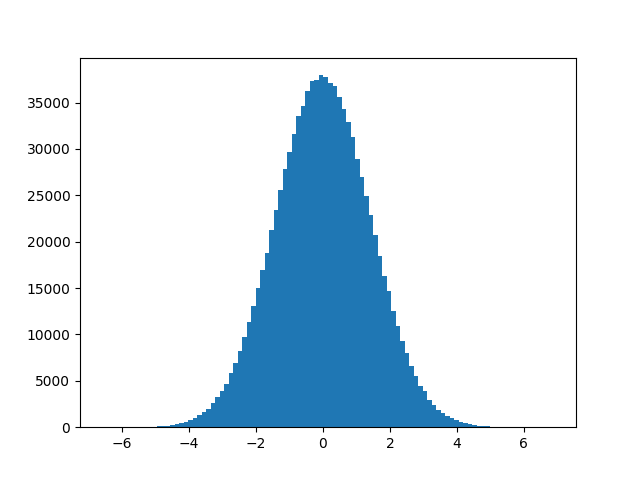
\includegraphics[width=\columnwidth]{solutions/2016/june/107/figures/norm.png}
\caption{Z when X is standard normal}
\label{june2016-107:fig:normal}
\end{figure}
\begin{figure}[!ht]
\centering
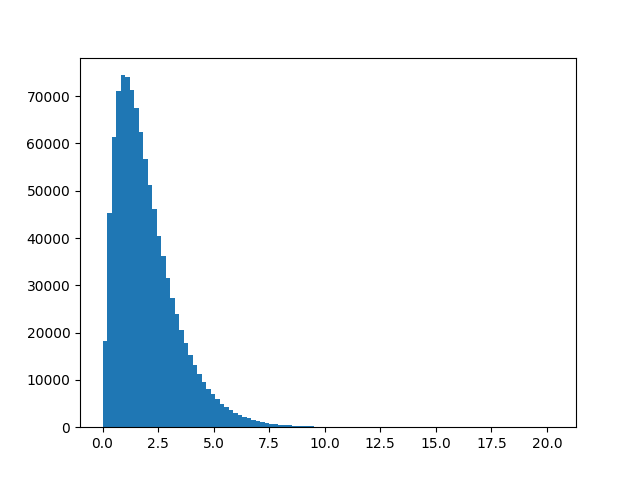
\includegraphics[width=\columnwidth]{solutions/2016/june/107/figures/expon.png}
\caption{Z when X is exponential with $\lambda = 1$}
\label{june2016-107:fig:exponential}
\end{figure}
\begin{figure}[!ht]
\centering
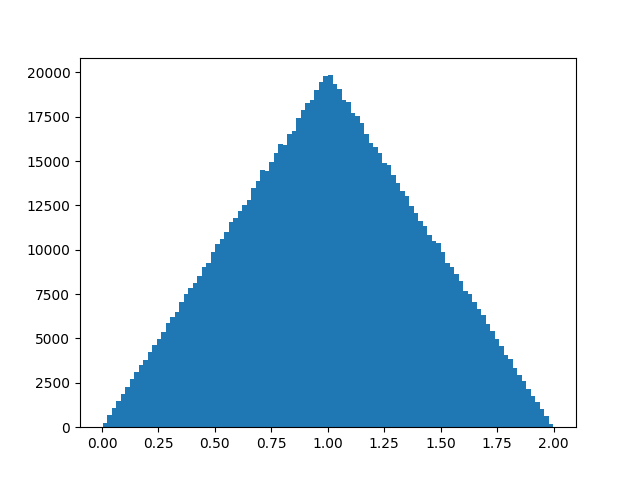
\includegraphics[width=\columnwidth]{solutions/2016/june/107/figures/uniform.png}
\caption{Z when X $\sim$ U(0,1)}
\label{june2016-107:fig:uniform}
\end{figure}
\begin{figure}[!ht]
\centering
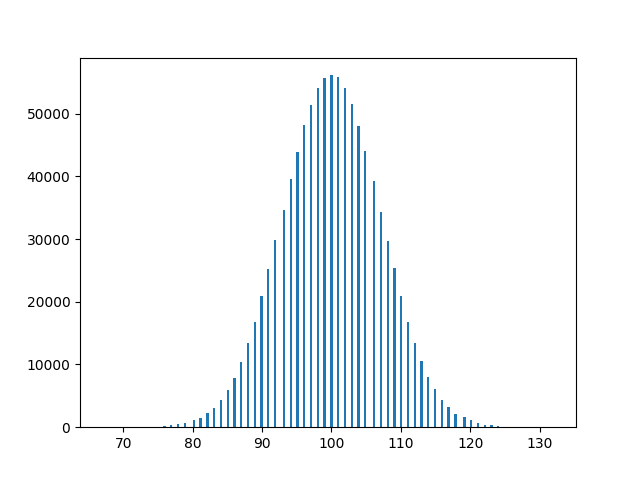
\includegraphics[width=\columnwidth]{solutions/2016/june/107/figures/binom.png}
\caption{Z when X $\sim$ B(100,0.5)}
\label{june2016-107:fig:binomial}
\end{figure}




\end{enumerate}